\documentclass[12pt,a4paper]{report}
\setlength\textwidth{145mm}
 \setlength\topmargin{0mm}
 \setlength\headsep{0mm}
 \setlength\headheight{0mm}
 
% Přepneme na českou sazbu
\usepackage[czech]{babel}
\usepackage[IL2]{fontenc}
\usepackage{graphicx} 

%% Použité kódování znaků: obvykle latin2, cp1250 nebo utf8:
\usepackage[utf8]{inputenc}
\begin{document}


\section{Náhodný testovací případ}
Oba testy (časový i krokový) jsme dělali na tabulkách velikosti $2097151$.
Pro graf s časy jsme průměrné doby průměrovali přes $58000$ insertů, je to hodnota,
při které se graf vyčistil na tolik, že bylo možné něco pozorovat. 
Násleující seznam přidává popis  k následujícím grafům.

\begin{itemize}
\item 1 -- linear probing with tabulation hash
\item 2 -- linear probing with multi hash
\item 3 -- linear probing with naive mod hash
\item 4 -- cucko with tabulation hash
\item 5 -- cucko with mult hash 
\end{itemize}
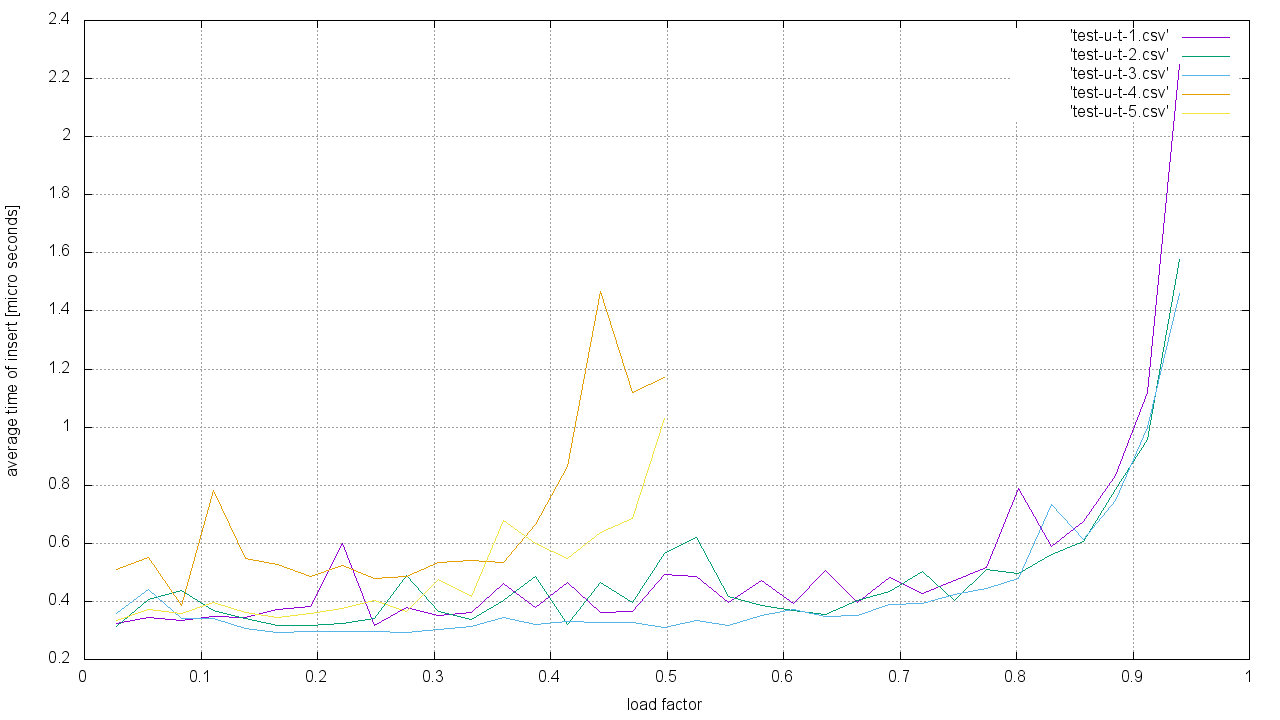
\includegraphics[width=\textwidth]{./tests/time_test/uniform-test.png}

Z grafu je překvapivě vidět, že naivní hashovací funkce potřebuje většinou
průměrně nejmenší dobu na insert. Pravděpodobně je to způsobeno jejím nejjednoduším výpočtem 
a zároveň přidáváním náhodných prvků z univerza.

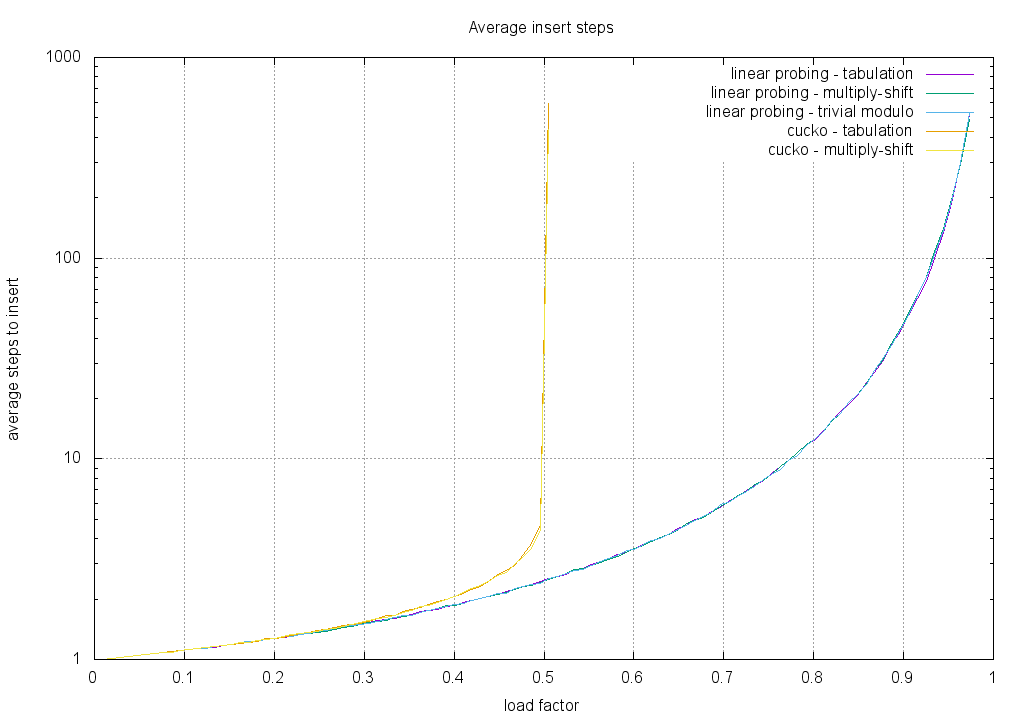
\includegraphics[width=\textwidth]{./tests/steps_test/uniform-test.png}

V obou grafech také vidíme, že u kukačky začne doba rychle stoupat už u z poloviny plné tabulky.
Pro druhý graf ukazující průměrný počet potřebných kroků byly hodnoty průměrovýny přes $10000$ vložení.
Není zde vidět žádnž rozdíl plynoucí z rozdílných hashovacích funkcí, což je zřejmě způsobeno tím, 
že vkládané prvky jsou zcela náhodné.


\section{Sekvenční testovací případ}

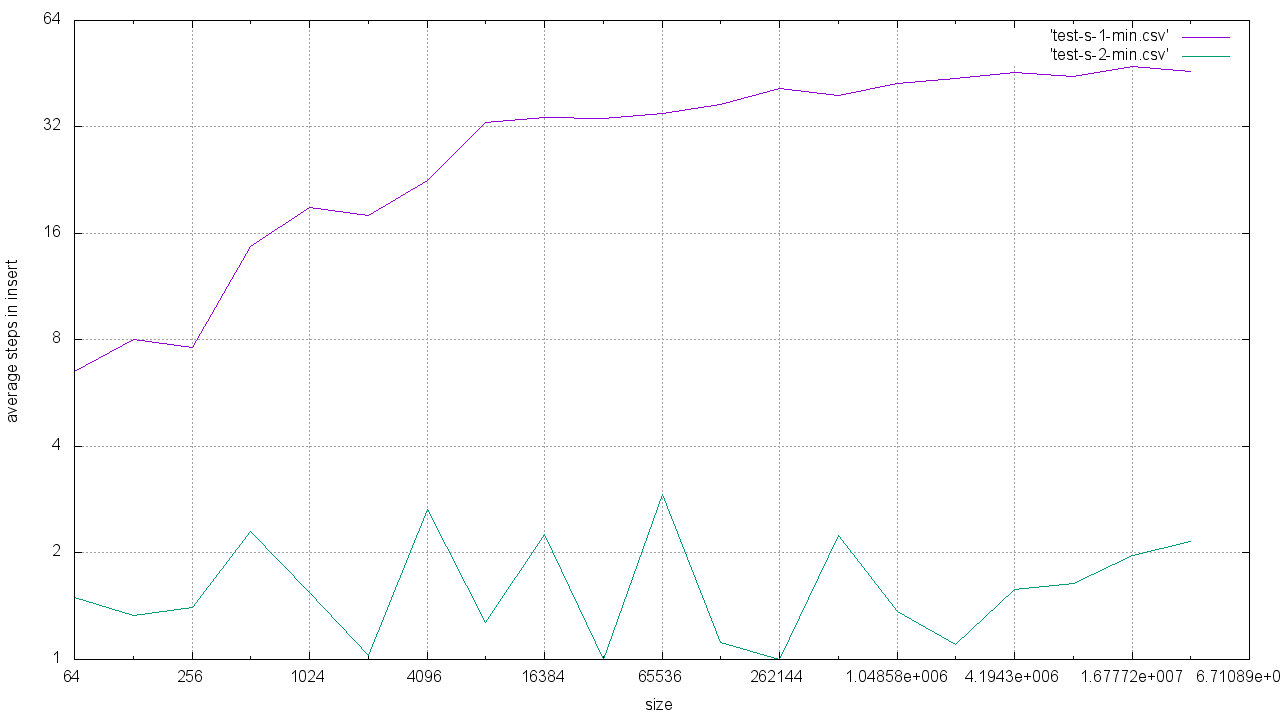
\includegraphics[width=\textwidth]{./tests/sequence_test/uniform-test1.png}
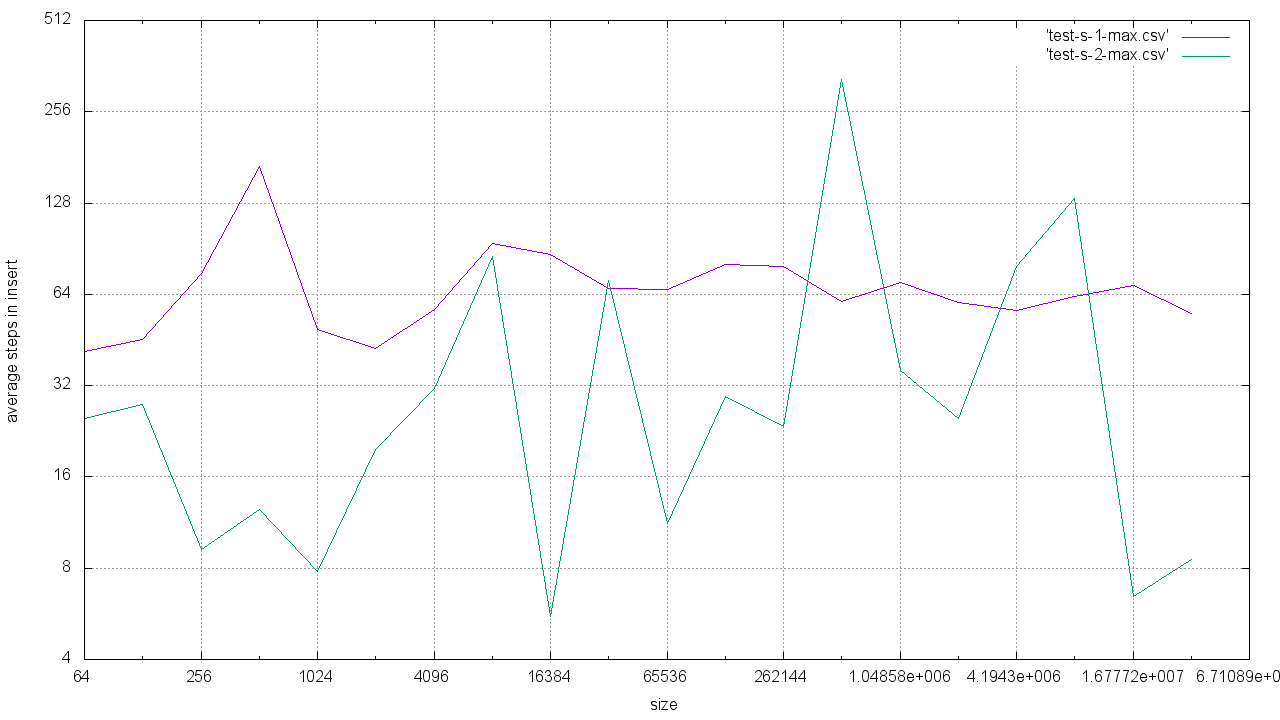
\includegraphics[width=\textwidth]{./tests/sequence_test/uniform-test2.png}
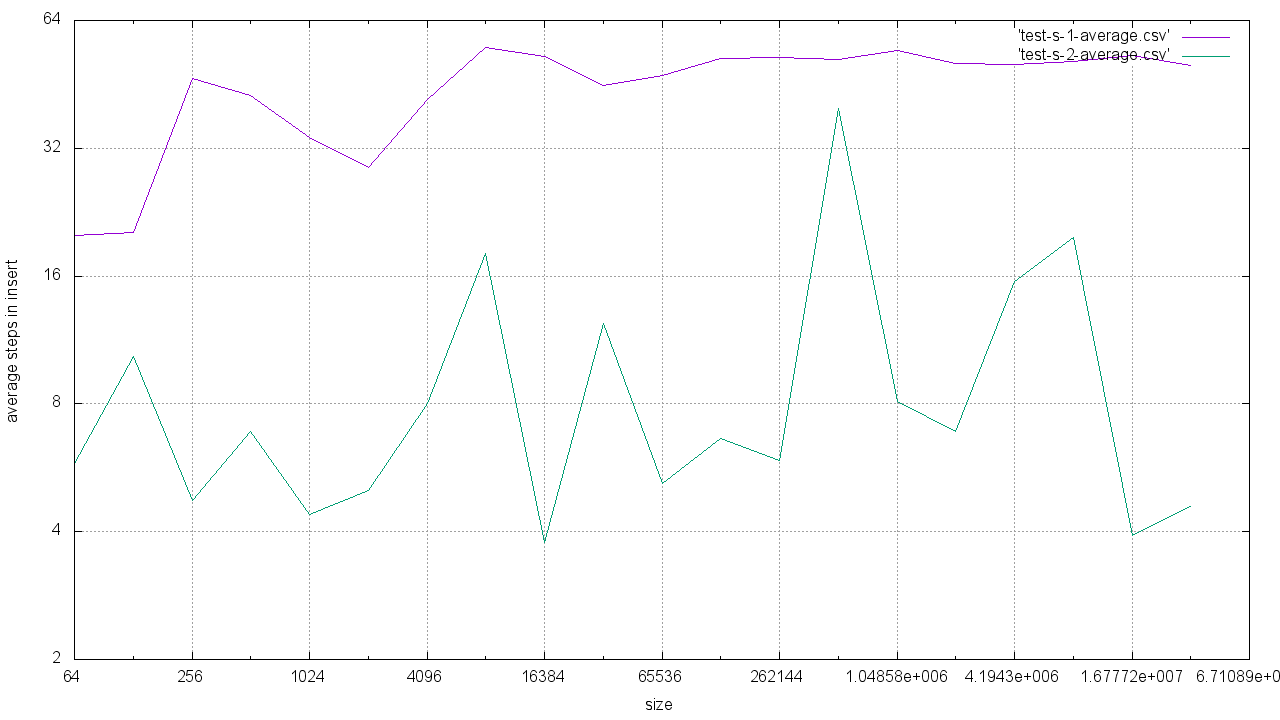
\includegraphics[width=\textwidth]{./tests/sequence_test/uniform-test3.png}
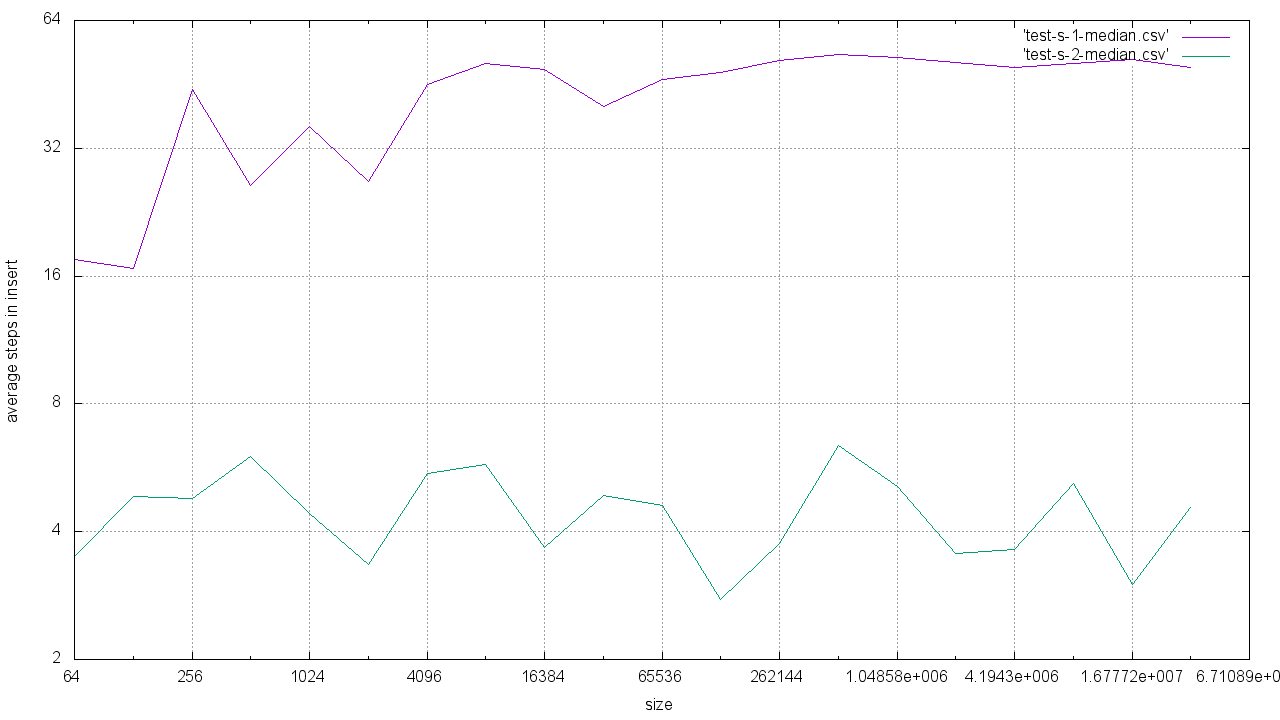
\includegraphics[width=\textwidth]{./tests/sequence_test/uniform-test4.png}
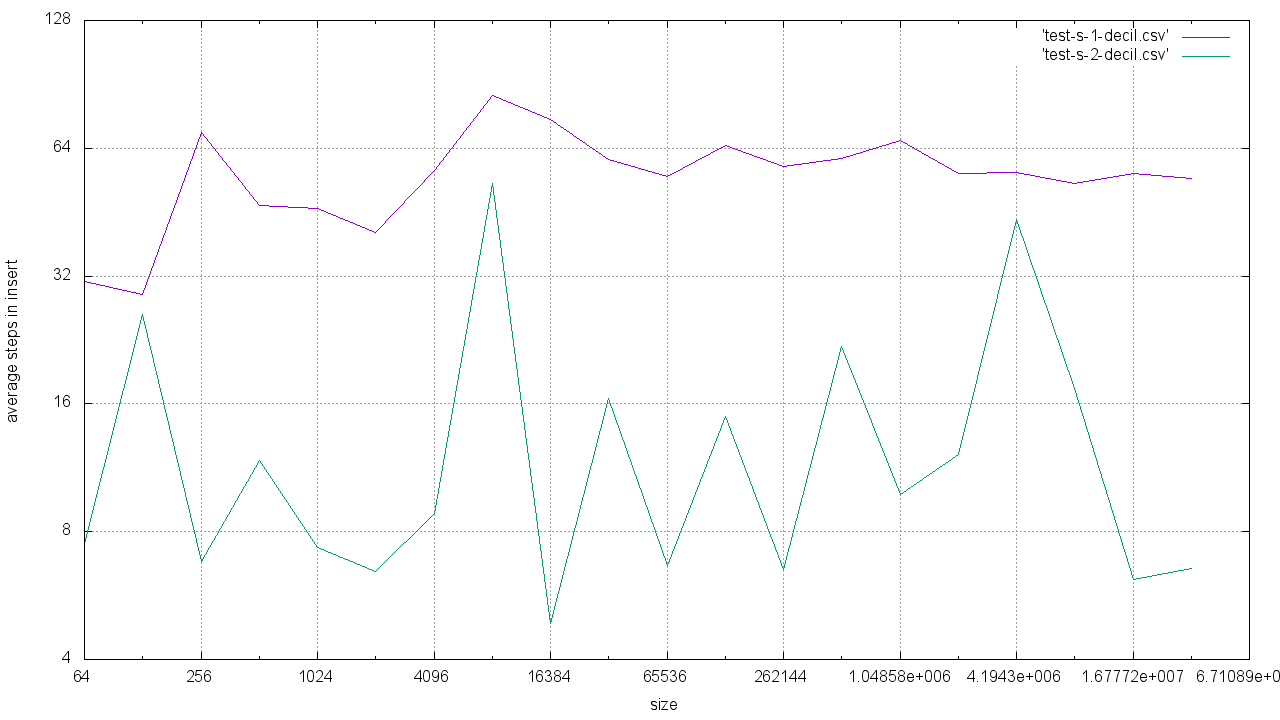
\includegraphics[width=\textwidth]{./tests/sequence_test/uniform-test5.png}





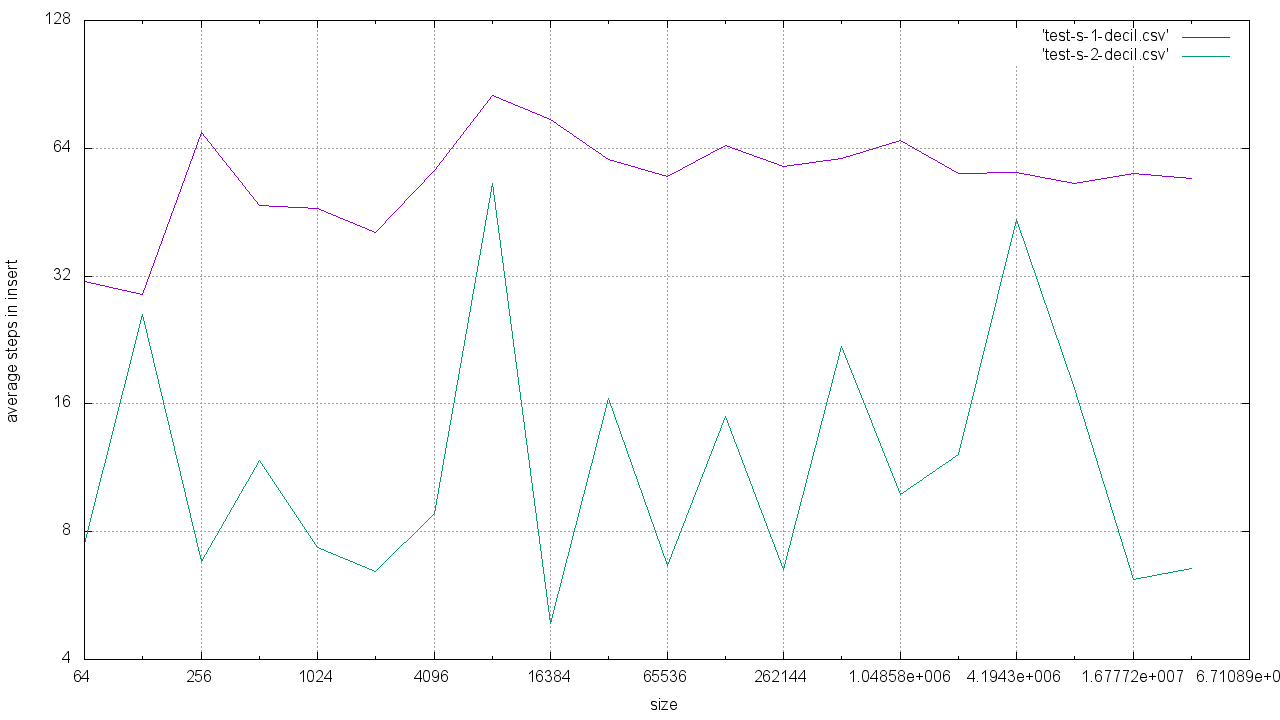
\includegraphics[width=\textwidth]{./tests/sequence_test/uniform-test.png}
  
\end{document}
